\section{Empirical Study of Evaluation Deviations}
\label{sec:empirical-study}

\subsection{Study Goal and Scope}

This empirical study characterizes the evaluation deviations and evaluation-affecting engineering factors reported in embodied AI and robot-learning projects. We study GitHub issues and pull requests as project-maintenance evidence of evaluation problems. These records capture developer-observed symptoms such as success-rate mismatches, rollout anomalies, evaluation crashes, reproduction failures, and unexpected benchmark behavior, together with suspected causes such as controller interfaces, reset states, simulator or runtime dependencies, checkpoint compatibility, observation preprocessing, and evaluation harness changes.

The goal of this study is to characterize the problem space rather than to estimate the prevalence of all embodied-AI bugs. Following empirical bug-study practice, we treat each retained record as evidence for a deviation symptom, an evaluation-affecting factor, an affected pipeline phase, and the strength of the explanatory evidence. This produces a taxonomy of symptoms and factors grounded in real project maintenance, and it also identifies the kinds of artifacts that a diagnosis method must explicitly reason about: manifests, run outcomes, episode-level behavior, failed executions, and cases where the available evidence is insufficient for attribution.

\subsection{Data Collection and Classification}

We mined GitHub issues and pull requests from 15 embodied-AI and robot-learning projects, including LeRobot, LIBERO, ManiSkill, Habitat-Sim, Habitat-Lab, ManiSkill-Learn, RLBench, robosuite, MetaWorld, CALVIN, OpenVLA, OFT, vla-evaluation-harness, Isaac Lab, and SimplerEnv. Keyword mining produced 2,714 candidates. A relevance screen assisted by a large language model retained 641 candidates about evaluation, benchmarking, rollout behavior, reproducibility, or evaluation-affecting factors. We then manually classified the screened candidates and retained 473 evidence records for the final taxonomy. The frozen JSON Lines (JSONL) record keeps the original repository, URL, issue or pull-request text, comments, matched keywords, human classification fields, and short evidence quotes.

Each retained record is classified by four dimensions: evidence role, primary deviation symptom, primary engineering factor, and affected pipeline phase. Evidence role records whether the report contains both a deviation and an explanatory factor, only a deviation, or only a factor that can plausibly change evaluation behavior. A single annotator manually classified the screened candidates, and the frozen records were then summarized deterministically; we use the study as problem evidence and taxonomy construction, not as a precise prevalence estimate over all embodied-AI maintenance.

The classification intentionally uses project-maintenance language rather than model-centric language. For example, an issue that reports a crash during reset is classified as an evaluation crash or failure, with reset or initial state as the factor if the thread identifies stale environment state as the cause. A pull request that changes controller semantics is classified by the action/controller interface factor even if it does not report a specific metric drop. This coding scheme preserves the engineering context that developers use when they triage benchmark changes and provides the factor vocabulary for the controlled evaluation matrix.

\begin{table}[!t]
  \caption{RQ1 Evidence Summary}
  \label{tab:rq1-summary}
  \centering
  \renewcommand{\arraystretch}{1.10}
  \begin{tabular}{lrr}
    \toprule
    Evidence role & Count & Percent \\
    \midrule
    Deviation and factor & 258 & 54.55\% \\
    Deviation only & 144 & 30.44\% \\
    Factor only & 71 & 15.01\% \\
    \midrule
    Total & 473 & 100.00\% \\
    \bottomrule
  \end{tabular}
\end{table}

\begin{figure}[t]
  \centering
  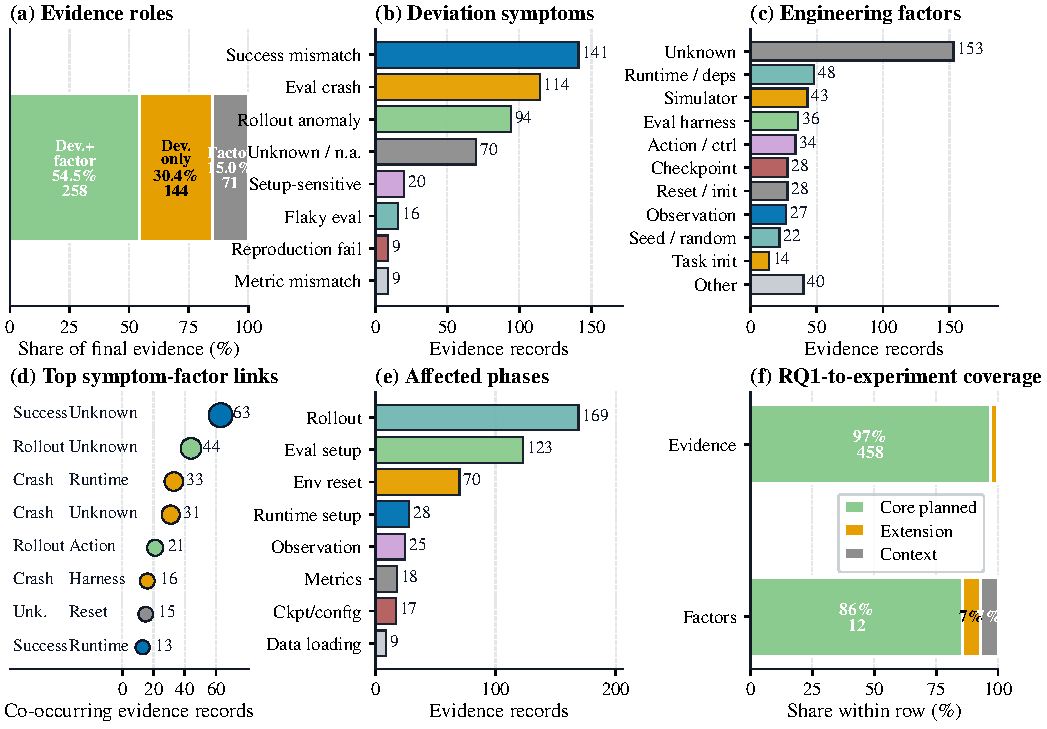
\includegraphics[width=\columnwidth]{figures/rq1_evidence_overview.pdf}
  \caption{RQ1 evidence overview: the panels summarize evidence roles, deviation symptoms, engineering factors, symptom--factor links, affected pipeline phases, and how the taxonomy maps to the controlled evaluation coverage.}
  \label{fig:rq1-evidence}
\end{figure}

\subsection{Results}

\noindent\textbf{Deviation symptoms.}
Figure~\ref{fig:rq1-evidence} and Table~\ref{tab:rq1-summary} show that evaluation deviations are not confined to one symptom type. Success-rate drops or mismatches account for 141 records, evaluation crashes or failures for 114 records, and rollout behavior anomalies for 94 records. The remaining records include setup-sensitive outcomes, instability or flakiness reports, reward/score mismatches, and reproduction failures. These categories span completed rollouts, failed executions, and reproduction problems, rather than a single aggregate metric.

\noindent\textbf{Finding~1.} Evaluation deviations are heterogeneous: real reports include aggregate metric changes, rollout anomalies, execution failures, and reproduction gaps.

\noindent\textbf{Engineering factors.}
The largest specified factor families include dependency/runtime environment, simulator/physics/rendering, evaluation script or harness behavior, action/controller interface, checkpoint/config compatibility, reset or initial state, and observation/sensor preprocessing. These factors often sit outside the learned policy itself. A changed benchmark result can therefore be associated with the evaluation stack, the task wrapper, or the controller interface even when the checkpoint is unchanged.

\noindent\textbf{Finding~2.} Many reported deviations are tied to evaluation-stack factors rather than to the policy checkpoint alone.

\noindent\textbf{Underspecified evidence.}
The factor \mbox{\emph{unknown\_or\_not\_specified}} appears in 153 of 473 records, or 32.35\%. These records often report a symptom without a confirmed causal factor, or mention configuration differences without enough behavioral evidence for causal attribution. This under-specification is part of the empirical phenomenon rather than an annotation error: project threads frequently stop after a workaround, reproduction gap, or partial diagnosis.

\noindent\textbf{Finding~3.} A substantial fraction of real reports lacks enough evidence for confident factor attribution.

\subsection{Implications for Controlled Evaluation}

These empirical observations shape the controlled LeRobot+LIBERO matrix in three ways. First, the matrix must include both completed-rollout and failed-run cases, because real reports include both metric deviations and execution failures. Second, the factor set must span the evaluation pipeline rather than focusing only on seed changes or policy checkpoints. Third, the evaluation must include negative calibration cases, because real project records often contain configuration differences that are not sufficient evidence for causal attribution. These implications determine the later RQ3 denominator split between paper-only cases, failed-run cases, negative calibration cases, and robustness cases.
